\section{Effective dynamics}

\subsection{Separable dynamics}

\begin{frame}{General solution}
    Separable unitary dynamics are of the form $\mcU_{t}=U_{1}^{t}\otimes U_{2}^{t}$. Since $\rho_{max}$ state is of the form $\rho_{A}\otimes\rho_{B}$. The effective evolved state looks like
    \begin{equation*}
        \rho\mapsto pU_{1}^{t}\rho_{A}(U_{1}^{t})^{\dag}+(1-p)U_{2}^{t}\rho_{B} (U_{2}^{t})^{\dag}.
    \end{equation*}
    The expected values of observables $\pauli{i}$ evolve as
    \begin{align*}
        \begin{split}
            \expval{\pauli{i}(t)}=&\frac{p\tanh(p\lambda)}{2}\Tr[\pauli{i}U_{1}^{t}(\paulivec{r_{\rho}})(U_{1}^{t})^{\dag}]\\
        &+\frac{p\tanh((1-p)\lambda)}{2}\Tr[\pauli{i}U_{2}^{t}(\paulivec{r_{\rho}})(U_{2}^{t})^{\dag}].
        \end{split}
      \end{align*}
\end{frame}

\begin{frame}{Two cases}
    \begin{columns}
        \begin{column}{0.5\textwidth}
            \begin{itemize}
                \item Asume $U_{1}= U_{2}=U$.
                \item Thanks to symmetry, the evolution may be factored as
                \begin{align*}
                    \rho(t)&=pU^{t}\rho_{A}(U^{t})^{\dag}+(1-p)U^{t}\rho_{B}(U^{t})^{\dag} \\
                    &=U^{t}(p\rho_{A}+(1-p)\rho_{B})(U^{t})^{\dag}\\
                    &=U^{t}\rho(0)(U^{t})^{\dag}.
                    \end{align*}
                \item The effective dynamics are    
                \begin{equation*}
                    \rho\mapsto U^{t}\rho(U^{t})^{\dag}.
                \end{equation*}
            \end{itemize}
        \end{column}
        \begin{column}{0.5\textwidth}
            \begin{itemize}
                \item Asume either $U_{1}=\Id$ or $U_{2}=\Id$.
                \item Let $r_{A}\hat{r}_{\rho}$ and $r_{B}\hat{r}_{\rho}$ be the Bloch vectors of $\rho_{A}$ and $\rho_{B}$. Let $O_{i}$ be the rotation induced by $U_{i}$
                \item If $U_{2}=\Id$ then:
                \begin{equation*}
                    r\hat{r}_{\rho}\mapsto O_{1}(r\hat{r}_{\rho}-(1-p)r_{B}\hat{r}_{\rho})+(1-p)r_{B}\hat{r}_{\rho}.
                \end{equation*}
                \item If $U_{1}=\Id$ then:
                \begin{equation*}
                    r\hat{r}_{\rho}\mapsto r\hat{r}_{\rho}+(1-p)(O_{2}(r_{B}\hat{r}_{\rho})-r_{B}\hat{r}_{\rho}).
                \end{equation*}
            \end{itemize}
        \end{column}
    \end{columns}
\end{frame}

\begin{frame}{Effect on the Bloch Sphere}
    \begin{figure}[h!]
        \centering
        \begin{subfigure}{0.32\textwidth}
            \centering
            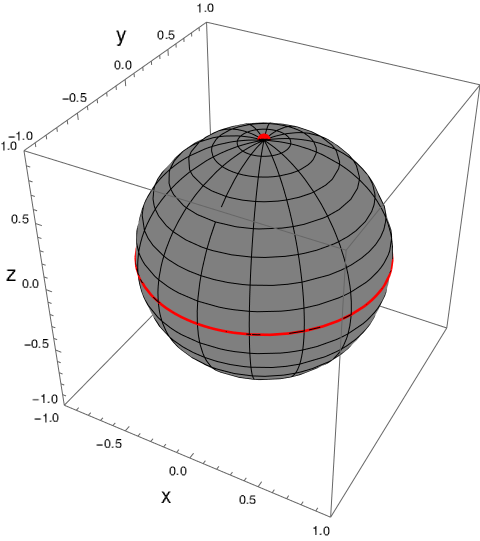
\includegraphics[width=0.9\linewidth]{figures/U1xU2_H1=Pi(sz)_H2=Id_z=0.9_p=0.6t=0.png}
            \caption{$t=0.0$}
        \end{subfigure}%
        \begin{subfigure}{0.32\textwidth}
            \centering
            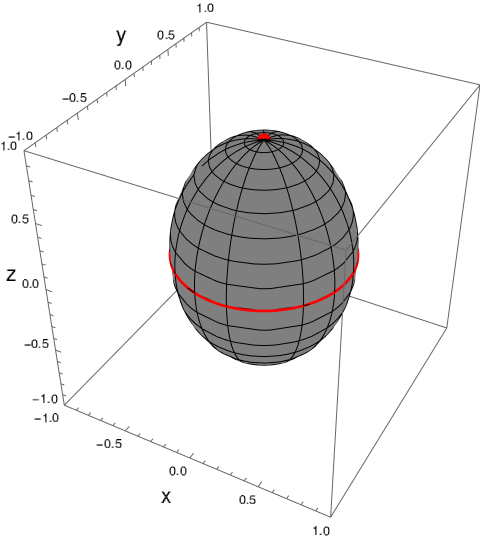
\includegraphics[width=0.9\linewidth]{figures/U1xU2_H1=Pi(sz)_H2=Id_z=0.9_p=0.6t=0.25.png}
            \caption{$t=0.25$}
        \end{subfigure}
        \begin{subfigure}{0.32\textwidth}
            \centering
            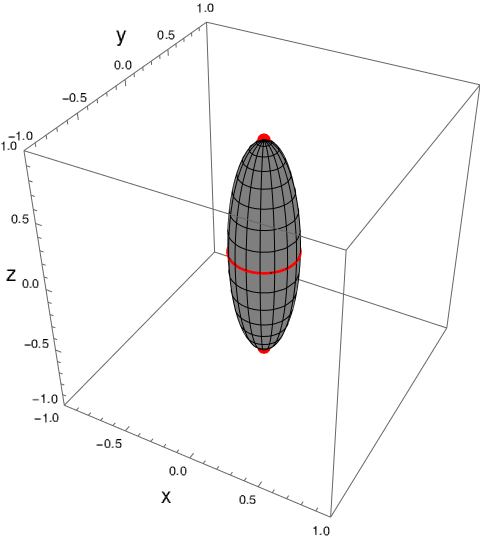
\includegraphics[width=0.9\linewidth]{figures/U1xU2_H1=Pi(sz)_H2=Id_z=0.9_p=0.6t=0.5.png}
            \caption{$t=0.5$}
        \end{subfigure}
        \caption{Effect on the Bloch sphere. $r=0.9$, $p=0.6$, $U_{1}=e^{it\pi \pauli{3}}$ and $U_{2}=\Id$}
    \end{figure}
\end{frame}



\begin{frame}{One example}
    \begin{columns}
        \begin{column}{0.5\textwidth}
            Let's consider an effective state
                \begin{equation*}
                    \rho=\frac{1}{2}(\Id+r_{z}\pauli{3}),
                \end{equation*}
            and an evolution $\mcU_{t}=e^{-itH_{1}}\otimes e^{-itH_{2}}$ where
                \begin{align*}
                    H_{1}=\pauli{3} & & \text{and} & & H_{2}=\frac{\omega}{\sqrt{2}}(\pauli{1}-\pauli{2}).
                \end{align*}
            We may solve this by using the formula
                \begin{equation*}
                    \rho\mapsto pU_{1}^{t}\rho_{A}(U_{1}^{t})^{\dag}+(1-p)U_{2}^{t}\rho_{B} (U_{2}^{t})^{\dag}.
                \end{equation*}
        \end{column}
        \begin{column}{0.5\textwidth}
            The unitaries might be written as
                \begin{equation*}
                    U_{1}^{t}=\Id\cos(\omega t) - i \pauli{3} \sin(\omega t),
                \end{equation*}
                \begin{equation*}
                    U_{2}^{t}=\Id\cos(\omega t) - \frac{i}{\sqrt{2}} (\pauli{1}-\pauli{2}) \sin(\omega t).
                \end{equation*}
                In a no-error scenario, we expect $\expval{\pauli{3}}=r_{z}$. Here, it is found to be:
                \begin{equation*}
                    \expval{\pauli{3}(t)}=\expval{\pauli{3}(0)}+(1-p)r_{B}(\cos(2\omega t)-1).
                \end{equation*}
            Note that $\expval{\pauli{3}(0)}$ is nothing but $r_{z}$.
        \end{column}
    \end{columns}
\end{frame}

\begin{frame}{Effect on the Bloch Sphere}
    \begin{figure}[h!]
        \centering
        \begin{subfigure}{0.44\textwidth}
            \centering
            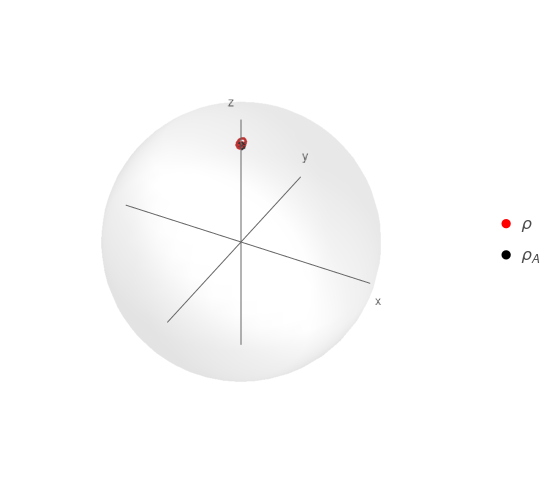
\includegraphics[width=0.9\linewidth]{figures/U1xU2_H1=(sz)_H2=15(sx-sy)_z=0.8_p=0.9_far.png}
        \end{subfigure}%
        \begin{subfigure}{0.44\textwidth}
            \centering
            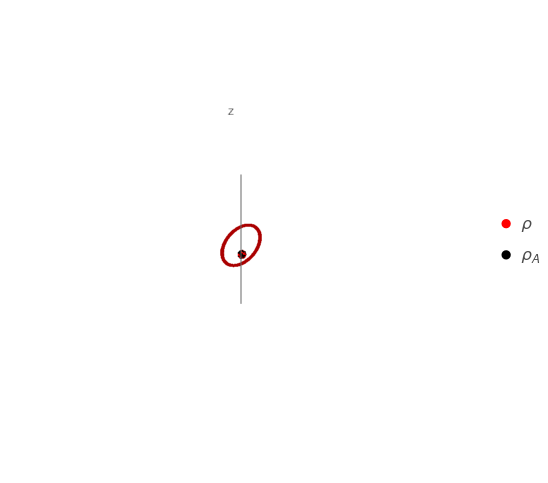
\includegraphics[width=0.9\linewidth]{figures/U1xU2_H1=(sz)_H2=15(sx-sy)_z=0.8_p=0.9.png}
        \end{subfigure}
        \caption{Graphical interpretation. The effective state $\rho$ oscillates near $\rho_{A}$, the subsystem of interest.}
    \end{figure}
\end{frame}

\begin{frame}{Other states}
    \begin{columns}
        \begin{column}{0.5\textwidth}
            This oscillation is observable even if the initial efective state, $\rho$, is not invariant under the unitary $U_{1}$.
            
            Let $\rho$ be
            \begin{equation*}
                \rho=\frac{1}{2}\qty[\Id+\frac{4}{5\sqrt{2}}\qty(\frac{1}{2}\pauli{1}+\frac{1}{2}\pauli{2}+\pauli{3})]
            \end{equation*}
            Clearly, this state is not invariant under 
            \begin{equation*}
                U_{1}^{t}=\Id\cos(\omega t) - i \pauli{3} \sin(\omega t).
            \end{equation*}
        \end{column}
        \begin{column}{0.5\textwidth}
            \begin{figure}[h!]
                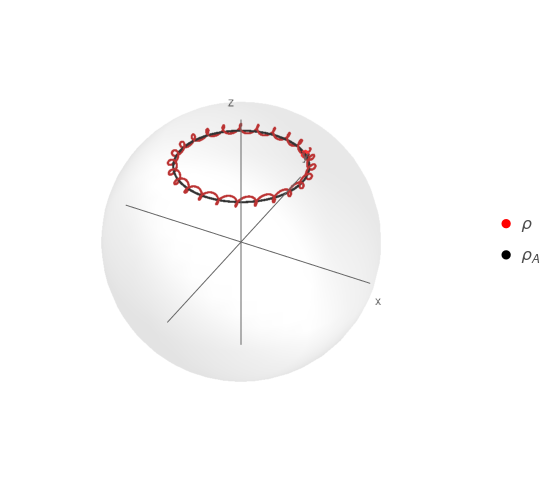
\includegraphics[width=0.8\columnwidth]{figures/U1xU2_H1=(sz)_H2=15(sx-sy)_z=0.8_p=0.9_wXY=0.5.png}%
                \caption{Small oscillations around the no-error trajectory. Here, $r=0.8$ $p=0.9$ and $\omega=15$. }
            \end{figure}
        \end{column}
    \end{columns}
\end{frame}



\subsection{Quantum computing gates}

\begin{frame}{Effective SWAP}
    State before and after the SWAP evolution is
    \begin{align*}
        \rho(0)&=\frac{1}{2}[\Id+(\hat{r}_{\rho}\cdot\vec{\sigma})(p\tanh{-\lambda p}+(1-p)\tanh{-\lambda (1-p)})],\\
        \rho(t=1)&=\frac{1}{2}[\Id+(\hat{r}_{\rho}\cdot\vec{\sigma})((1-p)\tanh{-\lambda p}+p\tanh{-\lambda (1-p)})].
        \end{align*}
    Both states have the same orientation, but different purity. The effective dynamics are described by a contraction of the Bloch sphere. Contraction factor depends on $\lambda(\rho)$:
    \begin{equation*}
        \kappa_{1}=\frac{r_{\rho(1)}}{r_{\rho(0)}}=\frac{(1-p)\tanh{\lambda p}+p\tanh{\lambda (1-p)}}{
          p\tanh{\lambda p}+(1-p)\tanh{\lambda (1-p)}}.
      \end{equation*}
      This evolution can be written as
      \begin{equation*}
        \boxed{\frac{1}{2}(\Id+\vec{r}_{\rho}\cdot\vec{\sigma}) \xrightarrow{S} \frac{1}{2}(\Id+\kappa_{1}^{\rho}\vec{r}_{\rho}\cdot\vec{\sigma})}
      \end{equation*}
\end{frame}

\begin{frame}{The contraction factor}
    \begin{figure}[h!]
        \centering
        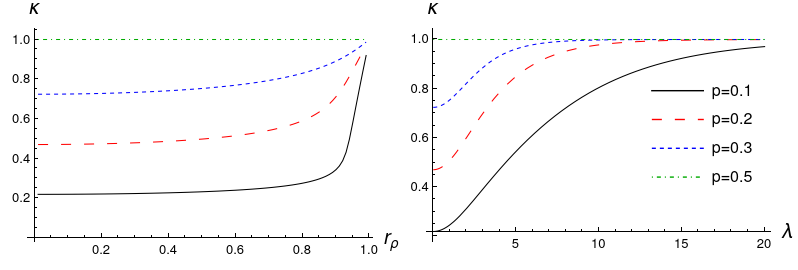
\includegraphics[width=0.9\linewidth]{figures/ContractionFactorSWAP_2D_both.png}
        \caption{$\kappa_{1}$ as a function of the initial purity $r_{\rho}$ (left) and as a function of the Lagrange multipliers $\lambda$ (right), for different values of $p$.}
        \label{fig:SWAPFactor2D}
      \end{figure}
\end{frame}

\begin{frame}{Generalized SWAP gate}
    SWAP gate might be extended to an arbitrary time as $S^{t}$. In this case, 
    \begin{equation*}
        \kappa_{t}^{\rho}=\frac{((1-p)\cos^{2}{\frac{\pi t}{2}}+p\sin^{2}{\frac{\pi t}{2}})\tanh{\lambda p}+(p\cos^{2}{\frac{\pi t}{2}}+(1-p)\sin^{2}{\frac{\pi t}{2}})\tanh{\lambda (1-p)}}{
          p\tanh{\lambda p}+(1-p)\tanh{\lambda (1-p)}}.
      \end{equation*}
      In terms of the spin observable $\sigma_{z}$, evolution looks like
\begin{equation}
  \expval{\sigma_{z}(t)}=\kappa_{t}^{\rho}\expval{\sigma_{z}(0)}.
\end{equation}
Or, in terms of the probability of getting either $\ket{0}$ or $\ket{1}$ as
 \begin{align}
  \bra{0}\rho(t)\ket{0}=\frac{1}{2}(1+\kappa_{t}^{\rho}\expval{\sigma_{z}(0)}) && \bra{1}\rho(t)\ket{1}=\frac{1}{2}(1-\kappa_{t}^{\rho}\expval{\sigma_{z}(0)}),
 \end{align}
 where both non linearity and time dependency is contained inside the contraction factor $\kappa_{t}^{\rho}$. 
\end{frame}
\begin{frame}{Effect on the Bloch sphere}
    \begin{figure}[h!]
        \centering
        \begin{subfigure}{0.32\textwidth}
            \centering
            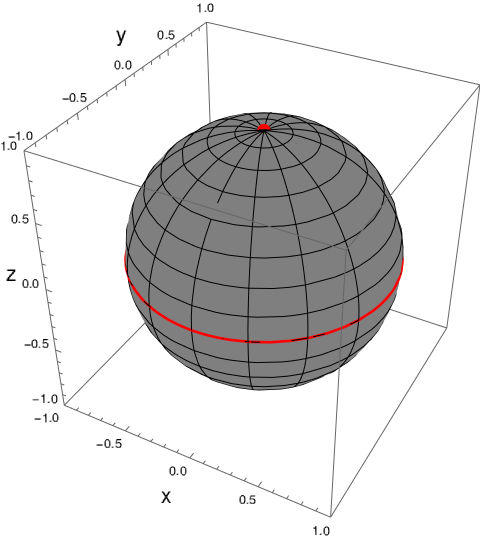
\includegraphics[width=0.9\linewidth]{figures/sphere_swapcontraction_t=0.0_z=0.9_p=0.9.png}
            \caption{$t=0.0$}
        \end{subfigure}%
        \begin{subfigure}{0.32\textwidth}
            \centering
            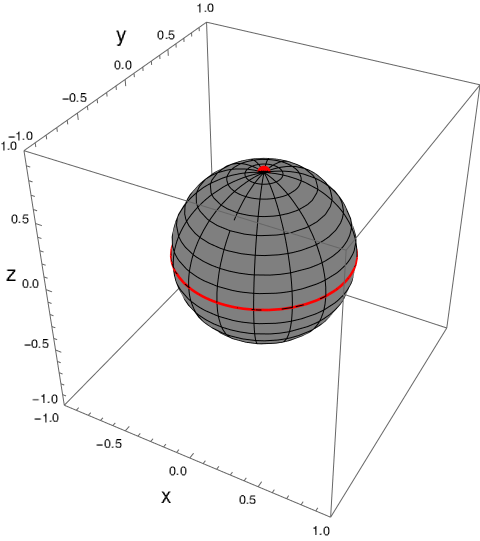
\includegraphics[width=0.9\linewidth]{figures/sphere_swapcontraction_t=0.5_z=0.9_p=0.9.png}
            \caption{$t=0.5$}
        \end{subfigure}
        \begin{subfigure}{0.32\textwidth}
            \centering
            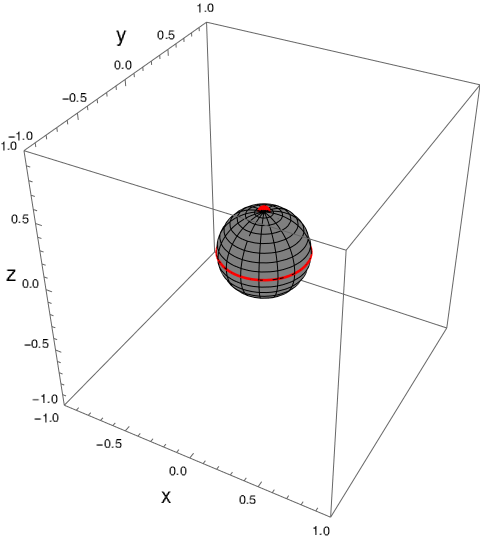
\includegraphics[width=0.9\linewidth]{figures/sphere_swapcontraction_t=1.0_z=0.9_p=0.9.png}
            \caption{$t=1.$}
        \end{subfigure}
        \caption{Effect on the Bloch sphere. $r=0.9$, $p=0.9$. The dramatic contraction can be associated with the near total loss of information.}
    \end{figure}
\end{frame}
\begin{frame}{Periodicity of the effective SWAP gate}
    \begin{figure}[h!]
        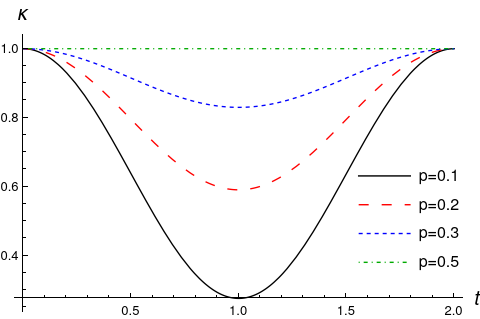
\includegraphics[width=0.5\columnwidth]{figures/ContractionFactorSWAP_z=0.8_t=0_to_t=2.png}%
        \caption{The contraction factor as a function of $t$, for different values of $p$ and $r=0.8$. Note the periodic nature of the effective evolution.}
    \end{figure}
\end{frame}


\begin{frame}{CNOT gate}
    The controlled not gatis generated by a hamiltonian
    \begin{equation*}
        H_{\cnot}=\frac{\pi}{4}\qty(\Id-\pauli{3}\otimes\Id-\Id\otimes\pauli{1}+\pauli{3}\otimes\pauli{1}),
    \end{equation*}
    From this, it is possible to expand the gate as three succesive unitary operators
    \begin{align*}
        \cnot&=e^{-i\frac{\pi}{4}\Id}e^{i\frac{\pi}{4}\pauli{3}\otimes\Id}e^{i\frac{\pi}{4}\Id\otimes\pauli{1}}e^{-i\frac{\pi}{4}\pauli{3}\otimes\pauli{1}}\\
        &=e^{-i\frac{\pi}{4}} (e^{i\frac{\pi}{4}\pauli{3}}\otimes \Id) (\Id \otimes e^{i\frac{\pi}{4}\pauli{1}}) e^{-i\frac{\pi}{4}\pauli{3}\otimes\pauli{1}}.
    \end{align*}
    While the usual CNOT interpretation of the gate might be blurry, another one arises: the CNOT gate induces correlations between the $\pauli{3}$ component of the first subsystem and the $\pauli{1}$ component of the second subsystem.
\end{frame}

\begin{frame}{Effective CNOT}
    Let's suppose for a moment than $p=1$. The evolved effective state will be
    \begin{equation*}
      \rho(t=1)=\rho(0)+\pauli{3}\rho(0)\pauli{3}=\frac{1}{2}(\Id+r_{3}\pauli{3}).
    \end{equation*}
    This is because the MaxEnt state will be $\rho\otimes\frac{1}{2}$. The $\pauli{1}$ and $\pauli{2}$ components are lost because the CNOT gate applies a $\pauli{3}$ gate on the first particle depending on the value of the second particle in the $\pauli{1}$ basis. If the second particicle finds itself on the state $\frac{1}{2}\Id$, the \textit{application rate} of the $\pauli{3}$ gate (that changes the $\pauli{1}$ and $\pauli{3}$ components) will be equally random: the information is lost.
\end{frame}

\begin{frame}{Effective CNOT}
    State before and after the SWAP evolution is
    \begin{align*}
        \rho(0)=&\frac{1}{2}[\Id+(\hat{r}_{\rho}\cdot\vec{\sigma})(p\tanh{-\lambda p}+(1-p)\tanh{-\lambda (1-p)})],\\
        \rho(t=1)=&\frac{1}{2}[p(\rho(0)+\sigma_{3}\rho_{A}\sigma_{3}+\Tr{\sigma_{1}\rho_{B}}[\rho_{A}-\sigma_{3}\rho_{A}\sigma_{3}])\\
    &+(1-p)(\rho(0)+\sigma_{1}\rho_{B}\sigma_{1}+\Tr{\sigma_{3}\rho_{A}}[\rho_{B}-\sigma_{1}\rho_{B}\sigma_{1}])].
        \end{align*}
    Notice the similarity between this expression and the previous one. The CNOT gate induces correlations between both subsystems. These corrleations are completely dependent on the $\pauli{3}$ and $\pauli{1}$ components of the first and second subsystem.
    The second term shows the action of the \textit{target} qubit over the \textit{control} qubit on the $\pauli{1}$ basis.
\end{frame}

\begin{frame}{Effective CNOT}
    State before and after the SWAP evolution is
    \begin{align*}
        \rho(0)=&\frac{1}{2}[\Id+(\hat{r}_{\rho}\cdot\vec{\sigma})(p\tanh{-\lambda p}+(1-p)\tanh{-\lambda (1-p)})],\\
        \rho(t=1)=&\frac{1}{2}[p(\rho(0)+\sigma_{3}\rho_{A}\sigma_{3}+\Tr{\sigma_{1}\rho_{B}}[\rho_{A}-\sigma_{3}\rho_{A}\sigma_{3}])\\
    &+(1-p)(\rho(0)+\sigma_{1}\rho_{B}\sigma_{1}+\Tr{\sigma_{3}\rho_{A}}[\rho_{B}-\sigma_{1}\rho_{B}\sigma_{1}])].
        \end{align*}
      This evolution can be written as
      \begin{equation*}
        \vec{r}_{\rho}=(pr_{A}+(1-p)r_{B})\hat{r}_{\rho}\mapsto\begin{pmatrix}
            r_{B}(pr_{A}(\hat{r}_{\rho,1})^2+(1-p)\hat{r}_{\rho,1})\\
            r_{B}r_{A}(p\hat{r}_{\rho,1}\hat{r}_{\rho,2}+(1-p)\hat{r}_{\rho,2}\hat{r}_{\rho,3})\\
            r_{A}(p\hat{r}_{\rho,3}+(1-p)r_{A}(\hat{r}_{\rho,3})^{2})
        \end{pmatrix}.
      \end{equation*}
\end{frame}

\begin{frame}{Effective CNOT on the Bloch sphere}
    \begin{figure}[h!]
        \centering
        \begin{subfigure}{0.32\textwidth}
            \centering
            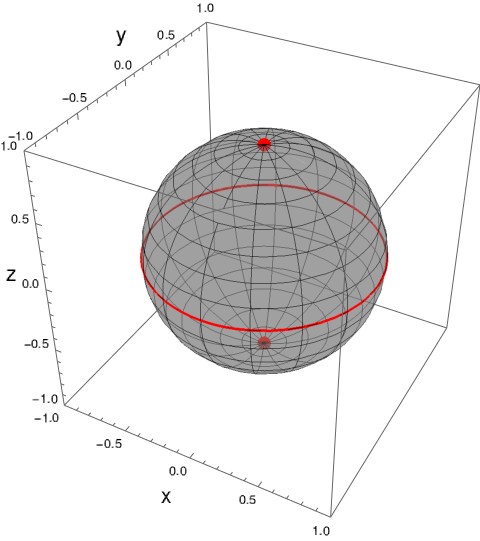
\includegraphics[width=0.9\linewidth]{figures/sphere_CNOT_t=0.0_z=0.8_p=0.95.png}
            \caption{$t=0.0$}
        \end{subfigure}%
        \begin{subfigure}{0.32\textwidth}
            \centering
            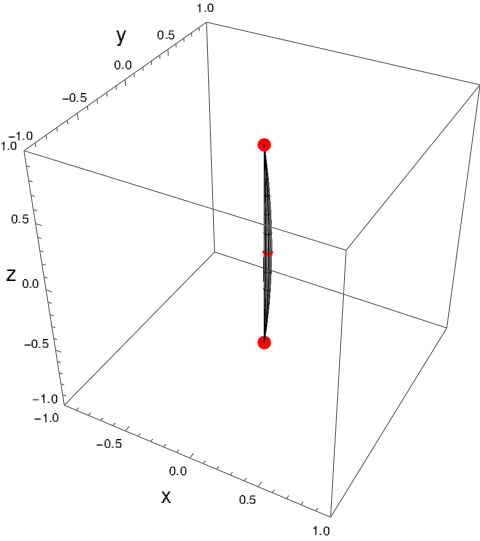
\includegraphics[width=0.9\linewidth]{figures/sphere_CNOT_t=1.0_z=0.8_p=0.95.png}
            \caption{$t=0.5$}
        \end{subfigure}
        \caption{Effect on the Bloch sphere. $r=0.8$, $p=0.95$.}
    \end{figure}
\end{frame}

\begin{frame}{Effective CNOT on the Bloch sphere}
    \begin{figure}[h!]
        \centering
        \begin{subfigure}{0.32\textwidth}
            \centering
            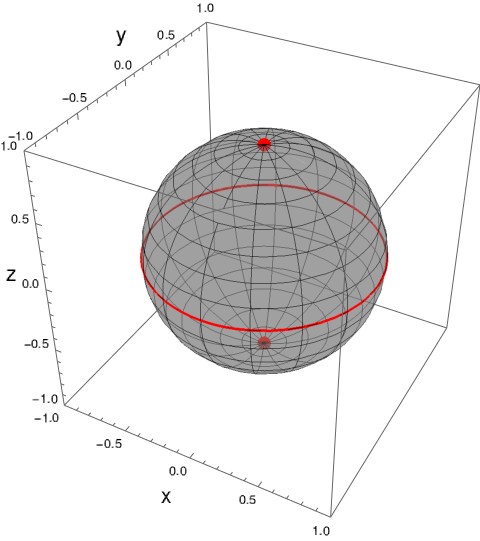
\includegraphics[width=0.9\linewidth]{figures/sphere_CNOT_t=0.0_z=0.8_p=0.6.png}
            \caption{$t=0.0$}
        \end{subfigure}%
        \begin{subfigure}{0.32\textwidth}
            \centering
            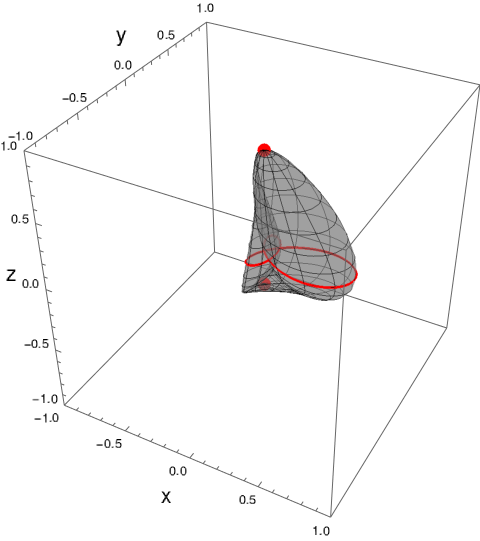
\includegraphics[width=0.9\linewidth]{figures/sphere_CNOT_t=1.0_z=0.8_p=0.6.png}
            \caption{$t=0.5$}
        \end{subfigure}
        \caption{Effect on the Bloch sphere. $r=0.8$, $p=0.6$.}
    \end{figure}
\end{frame}

\subsection{Special Dynamics}

\begin{frame}{Ising Model}
    We consider the following hamiltonian:
    \begin{align*}
        H=J\sigma_{z}\otimes\sigma_{z} && \Rightarrow && \mcU_{t}=\Id \cos{tJ} + i\sigma_{z}\otimes\sigma_{z}\sin{tJ}
    \end{align*}
    The evolved effective state looks like
    \begin{align*}
        \mcC{\varrho_{max}(t)}=&\rho(0)\cos^{2}{Jt}+\sigma_{3}\rho(0)\sigma_{3}\sin^{2}{Jt}\\
        &-i\frac{\lambda_{3}}{\lambda}\sin{Jt}\cos{Jt}[\sigma_{3},p\tanh((1-p)\lambda)\rho_{A}+(1-p)\tanh(p\lambda)\rho_{B}]
    \end{align*}
    Two important terms arise: the first is linear and independent of the coarse graining parameters, and the second one carries the non-linearity of the evolution, as it includes the Lagrange variable $\lambda$.
\end{frame}